\documentclass[12pt, a4paper]{article}
\renewcommand{\figurename}{Fig.}

\usepackage[utf8]{inputenc}
\usepackage{amssymb}
\usepackage{anyfontsize}
\usepackage{lipsum}
\usepackage{graphicx}
\usepackage{subcaption}
\usepackage{geometry}
\usepackage{tikz}
\usepackage{array}
\usepackage{enumitem}

%\usepackage[showframe]{geometry}

\usetikzlibrary{automata, positioning, arrows, calc}

\geometry{top      = 2cm,
		  bottom   = 2cm,
		  left     = 2cm,
		  right    = 2cm, 
		  footskip = 1cm}


% ----- STARTING DOCUMENT ----- %

\begin{document}

\pagenumbering{arabic}

\noindent
In the following, $p$ will be the parameter, $x$ and $y$ will be the clocks, $a$ and $b$ two natural numbers $\in \mathbb{N}$.\\

Tile forcing the following interval: $p \in (0, \frac{a}{2})$.

% In node, use accepting for initial states.
% In node, use fill=orange!50 for final states.
% In edge, use \cguard{} for guards.
% In edge, use \creset{} for assignments.

\begin{figure}[h!]
\newcommand{\cguard}{\textcolor{blue}}
\newcommand{\creset}{\textcolor{green!50!black}}

\begin{center}
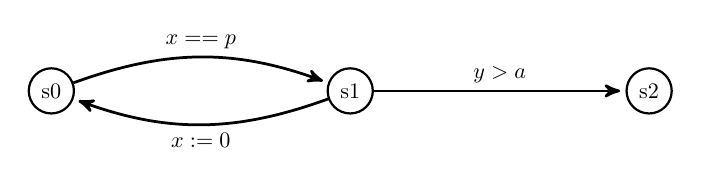
\begin{tikzpicture}[
	->,
	>=stealth',
	shorten >=2pt, 
	auto,
	scale=0.8,
    transform shape, 
    align=center,
    state/.style={thick, circle, draw}
    ] 
    
	\node[state] (s0) {s0};
	\node[state, right = 4cm of s0] (s1) {s1}; 
	\node[state, right = 4cm of s1] (s2) {s2}; 
		    
	\draw [line width=0.35mm]
	(s0) edge[bend left=20] node{\cguard{$x == p$}}(s1)
	(s1) edge[bend left=20] node{\creset{$x := 0$}} (s0)
	(s1) edge node{\cguard{$y > a$}} (s2)
    ;
\end{tikzpicture}
\end{center}

\caption{Loop Tile 1. Forced interval: $p \in (\frac{a}{2}, \infty)$}
\label{looptile 1}
\end{figure}


\bigskip

Tile forcing the following interval: $p \in (\frac{b}{2}, \infty)$.

% In node, use accepting for initial states.
% In node, use fill=orange!50 for final states.
% In edge, use \cguard{} for guards.
% In edge, use \creset{} for assignments.

\begin{figure}[h!]
\newcommand{\cguard}{\textcolor{blue}}
\newcommand{\creset}{\textcolor{green!50!black}}

\begin{center}
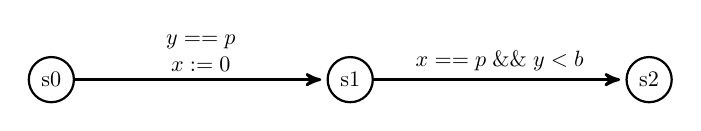
\begin{tikzpicture}[
	->,
	>=stealth',
	shorten >=2pt, 
	auto,
	scale=0.8,
    transform shape, 
    align=center,
    state/.style={thick, circle, draw}
    ] 
    
	\node[state] (s0) {s0};
	\node[state, right = 4cm of s0] (s1) {s1}; 
	\node[state, right = 4cm of s1] (s2) {s2}; 
		    
	\draw [line width=0.35mm]
	(s0) edge node{\cguard{$y == p$} \\ \creset{$x := 0$}}(s1)
	(s1) edge node{\cguard{$x == p \; \&\& \; y < b$}} (s2)
    ;
\end{tikzpicture}
\end{center}

\caption{Tile 2. Forced interval: $p \in (0, \frac{b}{2})$}
\label{tile 2}
\end{figure}



\noindent
The above tiles, namely Tile \ref{tile 1} and Tile \ref{tile 2}, can be considered as the basic building blocks for constructing every other interval, thanks to the possibility of chaining them together, hence restricting the interval in which the parameter $p$ will fall.\\

\noindent
The following one has been obtained by concatenating the aforementioned tiles.\\

Tile forcing the following interval: $p \in (\frac{a}{2}, \frac{b}{2})$.

% In node, use accepting for initial states.
% In node, use fill=orange!50 for final states.
% In edge, use \cguard{} for guards.
% In edge, use \creset{} for assignments.

\begin{figure}[h!]
\newcommand{\cguard}{\textcolor{blue}}
\newcommand{\creset}{\textcolor{green!50!black}}

\begin{center}
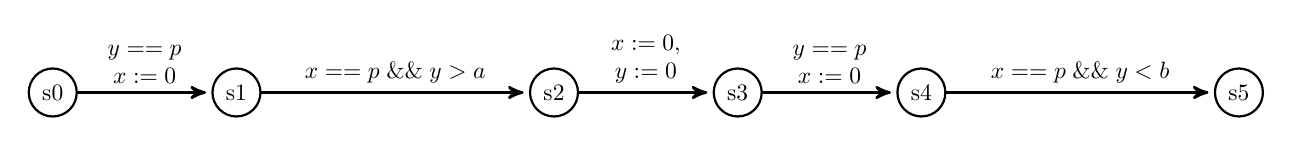
\begin{tikzpicture}[
	->,
	>=stealth',
	shorten >=2pt, 
	auto,
	scale=0.85,
    transform shape, 
    align=center,
    state/.style={thick, circle, draw}
    ] 
    
	\node[state] (s0) {s0};
	\node[state, right = 2cm of s0] (s1) {s1}; 
	\node[state, right = 4cm of s1] (s2) {s2}; 
	\node[state, right = 2cm of s2] (s3) {s3};
	\node[state, right = 2cm of s3] (s4) {s4};
	\node[state, right = 4cm of s4] (s5) {s5};   
		    
	\draw [line width=0.35mm]
	(s0) edge node{\cguard{$y == p$} \\ \creset{$x := 0$}}(s1)
	(s1) edge node{\cguard{$x == p \; \&\& \; y > a$}} (s2)
	(s2) edge node{\creset{$x := 0,$} \\ \creset{$y := 0$}} (s3)
	(s3) edge node{\cguard{$y == p$} \\ \creset{$x := 0$}}(s4)
	(s4) edge node{\cguard{$x == p \; \&\& \; y < b$}} (s5)
    ;
\end{tikzpicture}
\end{center}

\caption{Tile 3}
\label{tile 3}
\end{figure}



\noindent
Please note that Tile \ref{tile 3} can be written more concisely without using concatenation.\\

Tile forcing the following interval: $p \in (\frac{a}{2}, \frac{b}{2})$.

% In node, use accepting for initial states.
% In node, use fill=orange!50 for final states.
% In edge, use \cguard{} for guards.
% In edge, use \creset{} for assignments.

\begin{figure}[h!]
\newcommand{\cguard}{\textcolor{blue}}
\newcommand{\creset}{\textcolor{green!50!black}}

\begin{center}
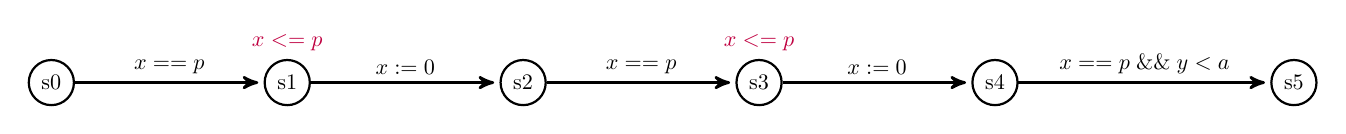
\begin{tikzpicture}[
	->,
	>=stealth',
	shorten >=2pt, 
	auto,
	scale=0.8,
    transform shape, 
    align=center,
    state/.style={thick, circle, draw}
    ] 
    
	\node[state] (s0) {s0};
	\node[state, right = 3cm of s0, label={[text=purple]$x <= p$}] (s1) {s1}; 
	\node[state, right = 3cm of s1] (s2) {s2};
	\node[state, right = 3cm of s2, label={[text=purple]$x <= p$}] (s3) {s3};
	\node[state, right = 3cm of s3] (s4) {s4};
	\node[state, right = 4cm of s4] (s5) {s5};

	\draw [line width=0.35mm]
	(s0) edge node{\cguard{$x == p$}} (s1)
	(s1) edge node{\creset{$x := 0$}} (s2)
	(s2) edge node{\cguard{$x == p$}} (s3)
	(s3) edge node{\creset{$x := 0$}} (s4)
	(s4) edge node{\cguard{$x == p \; \&\& \; y < a$}} (s5)
    ;
\end{tikzpicture}
\end{center}

\caption{Arbitrary interval Tile 4}
\label{arbitrary interval tile 4}
\end{figure}



\end{document}
